% !TEX spellcheck = en_US
% !TEX spellcheck = LaTeX
\documentclass[letterpaper,english,10pt]{article}
\usepackage{%
	amsfonts,%
	amsmath,%	
	amssymb,%
	amsthm,%
	babel,%
	bbm,%
	%biblatex,%
	caption,%
	centernot,%
	color,%
	enumerate,%
	%enumitem,%
	epsfig,%
	epstopdf,%
	etex,%
	fancybox,%
	framed,%
	fullpage,%
	%geometry,%
	graphicx,%
	hyperref,%
	latexsym,%
	mathptmx,%
	mathtools,%
	multicol,%
	pgf,%
	pgfplots,%
	pgfplotstable,%
	pgfpages,%
	proof,%
	psfrag,%
	%subfigure,%	
	tikz,%
	times,%
	ulem,%
	url,%
	xcolor,%
	mathpazo
}

\definecolor{shadecolor}{gray}{.95}%{rgb}{1,0,0}
\usepackage[margin=1in,top=0.75in]{geometry}
\usepackage[mathscr]{eucal}
\usepgflibrary{shapes}
\usepgfplotslibrary{fillbetween}
\usetikzlibrary{%
  arrows,%
  backgrounds,%
  chains,%
  decorations.pathmorphing,% /pgf/decoration/random steps | erste Graphik
  decorations.text,% 
  matrix,%
  positioning,% wg. " of "
  fit,%
  patterns,%
  petri,%
  plotmarks,%
  scopes,%
  shadows,%
  shapes.misc,% wg. rounded rectangle
  shapes.arrows,%
  shapes.callouts,%
  shapes%
}

%\pgfplotsset{compat=newest} %<------ Here
\pgfplotsset{compat=1.11} %<------ Or use this one

\theoremstyle{plain}
\newtheorem{thm}{Theorem}[section]
\newtheorem{lem}[thm]{Lemma}
\newtheorem{prop}[thm]{Proposition}
\newtheorem{cor}[thm]{Corollary}
\newtheorem{clm}[thm]{Claim}

\theoremstyle{definition}
\newtheorem{axiom}[thm]{Axiom}
\newtheorem{defn}[thm]{Definition}
\newtheorem{conj}[thm]{Conjecture}
\newtheorem{exmp}[thm]{Example}
\newtheorem{exerc}[thm]{Exercise}
\newtheorem{assum}[thm]{Assumptions}

\theoremstyle{remark}
\newtheorem{rem}[thm]{Remark}
\newtheorem{note}[thm]{Note}

\newcommand{\Cov}{\operatorname{Cov}}
%\newcommand{\det}{\operatorname{det}}
\newcommand{\Real}{\mathbb{R}}
\newcommand{\tr}{\operatorname{tr}}
%\newcommand{\Var}{\operatorname{Var}}

\DeclareMathOperator{\sign}{sign}
%\renewcommand{\proof}[1]{\begin{proof}#1\end{proof}}
\newcommand{\EQ}[1]{\begin{equation*}#1\end{equation*}}
\newcommand{\EQN}[1]{\begin{equation}#1\end{equation}}
\newcommand{\eq}[1]{\begin{align*}#1\end{align*}}
\newcommand{\meq}[2]{\begin{xalignat*}{#1}#2\end{xalignat*}}
\newcommand{\norm}[1]{\left\lVert#1\right\rVert}
\newcommand{\abs}[1]{\left\lvert#1\right\rvert}
\newcommand{\expect}[1]{\mathbb{E}\left[{#1}\right]}
\newcommand{\prob}[1]{\mathbb{P}\left[{#1}\right]}
\newcommand{\given}{\; \big\vert \;} 
\newcommand{\set}[1]{\left\{#1\right\}} 
\newcommand{\indicator}[1]{\mathbb{1}_{\set{#1}}} 
\newcommand{\inner}[1]{\left\langle#1\right\rangle}
\newcommand{\red}[1]{\textcolor{red}{#1}} 
\newcommand{\E}[1]{\mathbb{E}\left[#1\right]}
\newcommand{\Var}[1]{\operatorname{Var}\left[#1\right]}

\newcommand{\D}{\mathbb{D}}
%\newcommand{\E}{\mathbb{E}}
\newcommand{\N}{\mathbb{N}}
\renewcommand{\P}{\mathbb{P}}
\newcommand{\Q}{\mathbb{Q}}
\newcommand{\R}{\mathbb{R}}
\newcommand{\Z}{\mathbb{Z}}

\newcommand{\bU}{\mathbf{1}}
\newcommand{\bx}{\mathbf{x}}

\newcommand{\cB}{\mathcal{B}}
\newcommand{\cC}{\mathcal{C}}
\newcommand{\cD}{\mathcal{D}}
\newcommand{\cF}{\mathcal{F}}
\newcommand{\cG}{\mathcal{G}}
\newcommand{\cH}{\mathcal{H}}
\newcommand{\cO}{\mathcal{O}}
\newcommand{\cT}{\mathcal{T}}
\newcommand{\cX}{\mathcal{X}}
\newcommand{\cY}{\mathcal{Y}}

\newcommand{\sA}{\mathscr{A}}
\newcommand{\sB}{\mathscr{B}}
\newcommand{\sC}{\mathscr{C}}
\newcommand{\sD}{\mathscr{D}}
\newcommand{\sE}{\mathscr{E}}
\newcommand{\sF}{\mathscr{F}}
\newcommand{\sG}{\mathscr{G}}
\newcommand{\sH}{\mathscr{H}}
\newcommand{\sL}{\mathscr{L}}
\newcommand{\dO}{\mathscr{O}}
\newcommand{\sS}{\mathscr{S}}
\newcommand{\sT}{\mathscr{T}}
\newcommand{\sX}{\mathscr{X}}
\newcommand{\sY}{\mathscr{Y}}
\newcommand{\sZ}{\mathscr{Z}}

% Debug
\newcommand{\todo}[1]{\begin{color}{blue}{{\bf~[TODO:~#1]}}\end{color}}

% a few handy macros

\renewcommand{\le}{\leqslant}
\renewcommand{\ge}{\geqslant}
\newcommand\matlab{{\sc matlab}}
\newcommand{\goto}{\rightarrow}
\newcommand{\bigo}{{\mathcal O}}
%\newcommand{\half}{\frac{1}{2}}
%\newcommand\implies{\quad\Longrightarrow\quad}
\newcommand\reals{{{\rm l} \kern -.15em {\rm R} }}
\newcommand\complex{{\raisebox{.043ex}{\rule{0.07em}{1.56ex}} \hskip -.35em {\rm C}}}


% macros for matrices/vectors:

% matrix environment for vectors or matrices where elements are centered
\newenvironment{mat}{\left[\begin{array}{ccccccccccccccc}}{\end{array}\right]}
\newcommand\bcm{\begin{mat}}
\newcommand\ecm{\end{mat}}

% matrix environment for vectors or matrices where elements are right justifvied
\newenvironment{rmat}{\left[\begin{array}{rrrrrrrrrrrrr}}{\end{array}\right]}
\newcommand\brm{\begin{rmat}}
\newcommand\erm{\end{rmat}}

% for left brace and a set of choices
%\newenvironment{choices}{\left\{ \begin{array}{ll}}{\end{array}\right.}
\newcommand\when{&\text{if~}}
\newcommand\otherwise{&\text{otherwise}}
% sample usage:
%  \delta_{ij} = \begin{choices} 1 \when i=j, \\ 0 \otherwise \end{choices}


% for labeling and referencing equations:
\newcommand{\eql}{\begin{equation}\label}
\newcommand{\eqn}[1]{(\ref{#1})}
% can then do
%  \eql{eqnlabel}
%  ...
%  \end{equation}
% and refer to it as equation \eqn{eqnlabel}.  


% some useful macros for finite difference methods:
\newcommand\unp{U^{n+1}}
\newcommand\unm{U^{n-1}}

% for chemical reactions:
\newcommand{\react}[1]{\stackrel{K_{#1}}{\rightarrow}}
\newcommand{\reactb}[2]{\stackrel{K_{#1}}{~\stackrel{\rightleftharpoons}
   {\scriptstyle K_{#2}}}~}


\makeatletter
\def\th@plain{%
  \thm@notefont{}% same as heading font
  \itshape % body font
}
\def\th@definition{%
  \thm@notefont{}% same as heading font
  \normalfont % body font
}
\makeatother
\date{}


\title{Lecture-20: The Random Code Ensemble cntd...}


\begin{document}
\maketitle

\section{Geometry}

The relevant geometry for binary error-correcting codes is that of \textbf{Hamming space}. 
The $N$-dimensional binary Hamming space is the metric space defined by the set  $\set{0,1}^N$ and the Hamming metric
\EQ{
d(x,z) \triangleq \sum_{i=1}^N\indicator{x_i \neq z_i}.
}
Let us define the distance enumerator of a code $\fC$, relative to the codeword $z$, to be
\EQ{
\cN_z(h) \triangleq \abs{\set{x \in \fC: d(x,z) = h}},~ h \in [N].
}
For $ z = x^{(m)}$, this quantity is closely related to the conditional probability of decoding error given that $x^{(m)}$ is sent.
For the RCE, the quantity $\cN_{X^{(0)}}(h)$ is a random variable and we can easily determine its expected value. 
In particular, we have 
\eq{
\E \cN_{X^{(0)}}(h) &= \E\sum_{m \in \set{0,1}^M}\indicator{d(X^{(0)}, X^{(m)}) = h} = \indicator{h=0} + \sum_{m \in \set{0,1}^M\setminus 0}P\set{d(X^{(0)}, X^{(m)}) = h}\\
&= \indicator{h=0} + \sum_{m \in \set{0,1}^M\setminus 0}2^{-N}\binom{N}{h} 
=  \indicator{h=0} + (2^M-1)2^{-N}\binom{N}{h} \le 2^{M-N}\binom{N}{h}
}
for $h  \ge 1$. 
For a non-negative integer random variable $Z$, one has $P\set{Z \ge 1} \le \E Z$ (Markov's inequality). 
This implies that
\EQ{
P\set{\cN_{X^{0}}(h) \ge 1} \le 2^{M-N}\binom{N}{h},~~h \ge 1.
}
Since $d(X^{(0)},X^{(m)})$ is invariant under translation, 
the uniform distribution of $X^{(m)}$ for $m \neq 0$ implies that this result is completely independent of $X^{(0)}$
To analyze the asymptotics, we choose $M=\lfloor RN\rfloor$ with $R \in (0,1)$ and $h = \lfloor\delta N\rfloor$ with
$\delta \in (0,1)$. 
The quantity $\delta$ is called the \textbf{normalized} distance or weight of the codeword. 
In this case, 
\EQ{
\binom{N}{\lfloor{\delta N\rfloor}} \stackrel{\cdot}{=} 2^{N\cH(\delta)}. 
}
implies that 
\EQ{
P\set{\cN_{X^{(0)}}(\lfloor \delta N\rfloor) \ge 1} \le \E\cN_{X^{(0)}}(\lfloor \delta N\rfloor) \stackrel{\cdot}{=} 2^{N(R-1+\cH(\delta))}. 
}
If $R-1+\cH(\delta) < 0$, then the probability that a random codeword has another codeword closer than distance $\delta N$ is decreasing exponentially fast to $0$. 
Thus, the typical minimum distance, which is called the \textbf{Gilbert-Varshamov distance} and denoted by $\delta_{GV}(R)$ is given by the smallest root of $R-1+\cH(\delta)$. 
For example, $\delta_{GV}(1/2) = 0.11$. 

The quantity $r_N(\delta) = \frac{1}{N}\log_2\cN_{X^{(0)}}(\lfloor\delta N\rfloor)$ is also important in the analysis of code ensembles. 
It is often called the \textbf{exponential growth rate} or \textbf{spectral shape} of the ensemble. 
For the RCE, one can also show that $r_N(\delta)$ is concentrated around its asymptotic expectation $r(\delta) \triangleq ?? R-1+\cH(\delta)$ for all $\delta$ such that $r(\delta) > 0$. 
In particular, for any $\epsilon > 0$ and all $\delta \in (\delta_{GV}(R), 1 - \delta_{GV}(R))$, we have
\EQ{
\lim_{N\to\infty}P\set{\abs{\frac{1}{N}\log_2\cN_{X^{(0)}}(\lfloor \delta N\rfloor) - r(\delta)}>\epsilon} = 0.
}
\section{The binary symmetric channel}
\begin{figure}[h!]
    \centering
    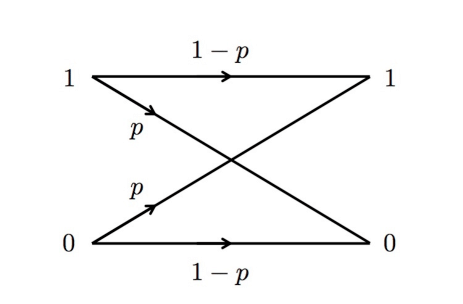
\includegraphics[scale=0.4]{Lectures/2019/Figures/bscp.png}
    \caption{Representation of BSC(p)}
    \label{fig:my_label}
\end{figure}
\flushleft The binary symmetric channel (BSC) with error probability $p$ is denoted by BSC($p$). 
This channel flips an input bit with probability $p$ and leaves it unchanged with probability $1 - p$. 
This implies that 
\EQ{
Q(y|x) = \begin{cases}
1-p, & x = y,\\
p, & x \neq y.
\end{cases}
}
\subsection{Word-MAP decoding}
For the BSC($p$) channel, we can rewrite the posterior probability distribution of input $x$ given observation $y$ as 
\EQ{
\mu_y(x)= \frac{1}{Z(y)}p^{d(x,y)}(1-p)^{N-d(x,y)}\frac{1}{\abs{\fC}}\indicator{x \in \fC} \propto \left(\frac{p}{1-p}\right)^{d(x,y)}\indicator{x \in \fC}.
}
Thus, if $p < 1/2$, the MAP codeword is precisely the codeword $x$ that minimizes the Hamming distance $d(x, y)$ (i.e., the closest codeword to the received sequence). 
Based on the geometry of the RCE, we know that w.h.p. the transmitted codeword is the unique codeword in a ball of radius $\delta_{GV}(R)N$ around the transmitted codeword. 
This also implies that, if we consider balls of radius $\delta_{GV}(R)N/2$ around each codeword, then only a vanishing fraction of these balls intersect each other. 
Thus, one can expurgate (i.e., delete) a vanishing fraction of codewords to make all of these balls are disjoint.\begin{figure}[h!]
    \centering
    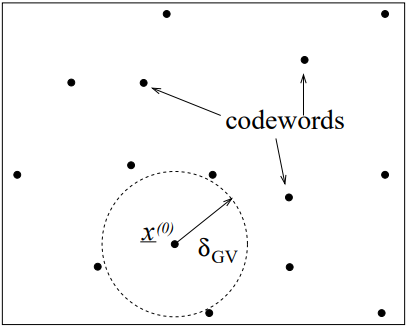
\includegraphics[scale=0.5]{Lectures/2019/Figures/RCE2.png}
    \caption{No codewords in $\delta_{GV}$ distance but exponentially many outside the hamming ball of radius $\delta_{GV}$ }
    \label{fig:my_label}
\end{figure}  
This expurgated code will correct all error patterns with fewer than $\delta_{GV}(R)N/2$ errors.
It turns out that one can actually handle twice as many errors. 


To see this, we observe two things. \\
First, the Hamming distance from the transmitted codeword to the received codeword $d(X^{(0)},Y)$ is a sum of i.i.d. Bernoulli-$p$ random variables and it satisfies the law of large numbers, 
\EQ{
\lim_{N\to\infty}P\set{\abs{\frac{1}{N}d(X^{(0)},Y) -p}>\epsilon}= 0.
}
Second, for any $\delta < \delta_{GV}(R)$, it holds that 
\EQ{
\lim_{N\to\infty}P\set{\frac{1}{N}\min_{m \in \set{0,1}^M\setminus 0}d(X^{(m)},Y)<\delta}= 0.
}
Since the analysis in the previous Section is independent of the distribution of $X^{(0)}$, 
this follows directly from analyzing the minimum distance of a code where $X^{(0)}$ is replaced by $Y$. 
Putting these together, we see that $p < \delta_{GV}(R)$ is sufficient w.h.p. for the correct codeword to be the closest codeword to the received vector. 
Applying $1 - \cH(\cdot)$ to both sides, 
this can be rewritten as $R < C_{BSC}(p) = 1- \cH(p)$ where $C_{BSC}(p)$ is the capacity of the BSC($p$). 
Thus, we have verified that the RCE achieves capacity on the BSC under Word-MAP decoding.
\begin{figure}
    \centering
    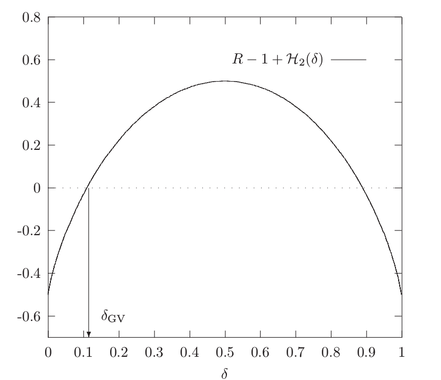
\includegraphics[scale=0.6]{Lectures/2019/Figures/RCE.png}
    \caption{Growth rate of the distance enumerator for the random code ensemble
with rate R = 1/2 as a function of the Hamming distance $d = N\delta$.}
    \label{fig:my_label}
\end{figure}

\section{Connections with statistical physics}
\subsection{The Random Energy Model}
The random energy model (REM) assumes the binary vectors ${0,1}^M$ are randomly associated with $2^M$ i.i.d. random variables drawn from a well-behaved distribution whose variance grows linearly with M (e.g., a Gaussian distribution with variance M/2).
For the BSC(p) channel with transmitted codeword $x = X^{(0)}$ and received vector y, the Hamming distances to incorrect codewords, 
\EQ{E_m= d(y,X^{(m)})\quad \text{for m} \neq 0,}
 are independent random variables with the binomial distribution
\EQ{P(E_m =k)= {\frac{1}{2}}^N \binom{N}{k}}
Thus, the distance between the received vector and the closest incorrect codeword is given by
\EQ{\min_{m'\in \set{0,1}^M}E_m' }     
This quantity is exactly the ground state energy of the  Random Energy Model with the binomial energy dis- tribution. When normalized by 1/N, this energy concentrates around the value $\delta_{GV}(R)$. Similarly, the distance between the received vector and the correct codeword, when normalized by 1/N, concentrates around the value p. Thus, \textbf{decoding will be successful if and only if} 
\EQ{p < \delta_{GV}(R)}.
\subsection{The Boltzmann Distribution}
Suppose we think about the decoding problem as a spin system where the energy of configuration x is given by
\EQ{
E(x) = \begin{cases}
-ln(Q(y/x)), & x \in \fC,\\
\infty, & otherwise.
\end{cases}
}
In this case, the Boltzmann distribution for inverse temperature is given by
\EQ{\mu_{\beta}(x)=\frac{1}{z(\beta)}e^{-\beta E(x)}=\frac{{Q(y/x)}^\beta}{z(\beta)}
}

\end{document}

